\subsubsection{Cancellation} The Cancellation axis defines how a running task is cancelled, including how cancellation is signaled, if at all, and how cancellation propagates between task dependencies. A clear cancellation mechanism is what distinguishes async/await from other concurrency paradigms. Within the cancellation axis there are two design dimensions: \textit{cooperation,} and \textit{direction.}

\ggnote{This section has not been updated}

In this section we will illustrate cancellation using the function \code{process} defined in \Cref{fig:cancellation} in both Rust (SMOL) and Python (AsyncIO).

\begin{figure}
  \begin{minipage}[t]{0.49\textwidth}
\begin{lstlisting}[language=Rust, linebackgroundcolor={\lineEq{15}}]
async fn process(
  db: Database,
  cache: Cache,
  request: Request,
) -> Response {
  let response = compute_response(
    &db, &cache, request).await;

  let db_update = smol::spawn(
    update_db(&db, &response));

  let cache_update = smol::spawn(
    update_cache(&cache, &response));

    db_update.await;
    cache_update.await;

  response
}
  \end{lstlisting}
  \end{minipage}\hfill%
  \begin{minipage}[t]{0.49\textwidth}
\begin{lstlisting}[language=Python, linebackgroundcolor={\lineEq{11}}]
async def process(db, cache, request):
  response = await compute_response(
    db, cache, request)

  db_update = asyncio.create_task(
    update_db(db, response))

  cache_update = asyncio.create_task(
    update_cache(cache, response))

  await db_update
  await cache_update

  return response
\end{lstlisting}
  \end{minipage}
  \cprotect\caption{An illustrative async function, \code{process}, that processes a request, and in turn, updates a database and cache in parallel. It's important that the cache and database remain in sync, but the chosen cancellation policy may break this invariant. (Left) A Rust implementation using the SMOL async framework. SMOL uses a top-down, non-cooperative cancellation policy that may leave the database and cache in a \textit{partially-updated} state. (Right) A Python implementation using the Asyncio library. Asyncio uses a bottom-up, cooperative cancellation policy that may leave the database unchanged and the cache fully updated.}
  \label{fig:cancellation}
\end{figure}

\paragraph{Cooperation} The Cooperation cancellation axis defines if cancellation requires cooperation from all tasks in the cancelled subtree. If cancellation is \textit{cooperative,} this means that a cancellation signal can get intercepted by a node in the tree if they do not cooperate. Cancellation is \textit{non-}cooperative if tasks have no choice but to cooperate with cancellation; non-cooperative cancellation can otherwise be referred to as termination.

In Rust a \Coro{} is represented as an enumeration. Cancelling an \Coro{} is defined by simply freeing the value's memory. In the asynchronous framework SMOL, a \Task{} can be cancelled by either invoking the \code{.cancel()} method or freeing the \Task{}, which in turn frees the underlying \Coro{}. As a consequence of Rust's choice to define cancellation as a memory free, it is not possible for an asynchronous function to prevent a cancellation. A memory free cannot be shielded or intercepted. Therefore, we classify Rust's cancellation as non-cooperative. Note that this cancellation policy remains non-cooperative regardless of the async framework chosen for a specific program.

\begin{figure}
  \begin{minipage}[t]{0.49\linewidth}
    \includegraphics[width=0.99\textwidth]{example-image-a}
  \end{minipage}\hfill%
  \begin{minipage}[t]{0.49\linewidth}
    \includegraphics[width=0.99\textwidth]{example-image-b}
  \end{minipage}
  \cprotect\caption{Example execution of the \code{process} function shown in \Cref{fig:cancellation}. (Left) The Rust (SMOL) implementation uses the non-cooperative memory free cancellation protocol. Both the \code{db_update} and \code{cache_udpate} are terminated, leaving the systems in a potentially inconsistent state. (Right) The Python (Asyncio) implementation uses exceptions to signal cancellation and the \code{cache_update} is left orphaned because cancellation is not signaled to it.}
  \label{fig:cancellation:swimlane}
\end{figure}

Shown in \Cref{fig:cancellation:swimlane}, if the executing Rust function \code{process} is cancelled at line fifteen, then the memory for \code{process}, \code{db_update}, and \code{cache_update} are all freed. Neither the database update nor the cache update can rollback partially-made changes, so unless both operations completed fully before the cancellation, the system is left in an inconsistent state.

Cancellation in Python is handled by raising an exception at the next await point blocking the task. Refering to the code in \Cref{fig:cancellation}, if the \code{process} function is cancelled at line eleven, the exception will be raised at an await point within the \code{update_db} function. Because \code{process} is waiting on \code{db_update}, an await point blocking the task is within the dynamic extent of \code{update_db}. The \textit{expectation} is that \code{update_db} will allow the exception to propagate, or reraise the exception if it needs to do some cleanup.

\begin{wrapfigure}{r}{0.35\textwidth}
  \raggedright
\begin{lstlisting}[language=Python,numbers=none]
async def db_update(db r):
  snap = await db.snapshot()
  try:
    # .. cancelled in here ..
  except:
    await db_rollback(snap)
\end{lstlisting}
  \cprotect\caption{An example of a Python function swalling a cancellation request. The function \code{db_update} is not cooperating in the cancellation protocol by using a try/except block, which catches all exceptions.}
  \label{fig:cancellation:cooperative}
\end{wrapfigure}

The \code{db_update} function may choose to, or be mistakenly programmed to, not cooperate with cancellation. \Cref{fig:cancellation:cooperative} provides an illustrative implementation of the \code{db_update} function that does not cooperate with the Asyncio cancellation protocol. A \code{asyncio.CancellationError} will get raised within the \code{db_update} function, however, since the function body is wrapped in a try/except block, the cancellation request is never propagated to the \code{process} function. \code{process} is unaware that the database was not updated and the database and cache are now out of sync.

\paragraph{Propagation direction} The Propagation Direction axis defines where in the waiting tree of dependencies cancellation is signaled first and how that signal is propagated to the rest of the waiting nodes. The possible values are \textit{top-down,} \textit{bottom-up,} and \textit{simultaneous.}

Before specifying exactly what the direction of cancellation propagation is, we first need to specify through what cancellation is propagating. Cancellation propagates through the \textit{task tree,} specifically, the task tree rooted at the cancelled task. Not all languages explicitly build a task tree in the runtime.

Consider the Rust (SMOL) code in \Cref{fig:cancellation}, at line fifteen, the set of tasks is depicted in \Cref{fig:cancellation:tree:rust}. Unlike Python, an edge between two tasks in the SMOL task tree is added when a task is \textit{spawned,} not when it's awaited. We say this because the calling task has ownership of the spawned task. When a task is cancelled, SMOL invokes the destructors as they would typically run in Rust, which flows down the tree represented by memory ownership. Therefore, we say that Rust (SMOL) cancellation propagates top-down.

\begin{wrapfigure}{l}{0.30\linewidth}
  {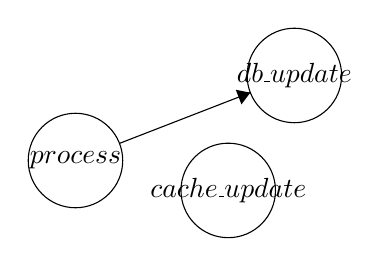
\begin{tikzpicture}[scale=0.2]
  \tikzstyle{every node}+=[inner sep=0pt]
    \draw [black] (13.3,-24.3) circle (3);
    \draw (13.3,-24.3) node {$\text{\tiny process}$};
    \draw [black] (27.2,-18.9) circle (3);
    \draw (27.2,-18.9) node {$\text{\tiny db\_update}$};
    \draw [black] (23,-26.2) circle (3);
    \draw (23,-26.2) node {$\text{\tiny cache\_update}$};
    \draw [black] (16.1,-23.21) -- (24.4,-19.99);
    \fill [black] (24.4,-19.99) -- (23.48,-19.81) -- (23.84,-20.74);
  \end{tikzpicture}
  \cprotect\subcaption{The state of the Python (Asyncio) task tree at line eleven. Because \code{process} is waiting on \code{db_update} the two form a tree, however, \code{cache_update} is not part of the current tree because it wasn't awaited.}
  \label{fig:cancellation:tree:python}}

  {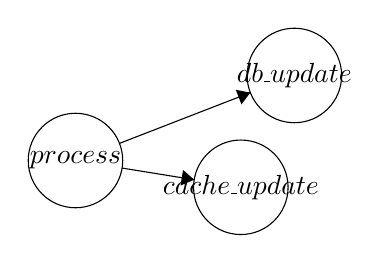
\begin{tikzpicture}[scale=0.2]
  \tikzstyle{every node}+=[inner sep=0pt]
  \draw [black] (13.3,-24.3) circle (3);
    \draw (13.3,-24.3) node {$\text{\tiny process}$};
  \draw [black] (27.2,-18.9) circle (3);
    \draw (27.2,-18.9) node {$\text{\tiny db\_update}$};
  \draw [black] (23.8,-26) circle (3);
    \draw (23.8,-26) node {$\text{\tiny cache\_update}$};
  \draw [black] (16.1,-23.21) -- (24.4,-19.99);
  \fill [black] (24.4,-19.99) -- (23.48,-19.81) -- (23.84,-20.74);
  \draw [black] (16.26,-24.78) -- (20.84,-25.52);
  \fill [black] (20.84,-25.52) -- (20.13,-24.9) -- (19.97,-25.89);
  \end{tikzpicture}
  \cprotect\subcaption{The state of the Rust (SMOL) task tree at line fifteen. Because SMOL's cancel on drop semantics, and Rust's owernship model, the task tree is help implicitly in Rust's memory.}
  \label{fig:cancellation:tree:rust}}

  \caption{The depicted task right before cancellation from the programs shown in \Cref{fig:cancellation}.}
  \label{fig:cancellation:tree}
\end{wrapfigure}

Consider the Python (Asyncio) code in \Cref{fig:cancellation}, at line 11, the set of tasks is depicted in \Cref{fig:cancellation:tree:python}. By default, all tasks in Asyncio are disjoint. Given two tasks, $A$ and $B$, where $B$ is spawned from within $A$, an edge in the task tree is added between the two nodes only when $A$ awaits $B$. Therefore, in our example program \code{db_update} is a child of \code{process} only because of the await present on line eleven. Therefore, cancellation is signalled from within \code{update_db}, and propagates \textit{upward} in the task tree to signal cancellation.

A \textit{simultaneous} cancellation would alert all tasks at the same time of cancellation. An example language with simultaneous cancellation propagation is Swift, as we will see in \Cref{sec:semantics}.

